%%%%%%%%%%%%%%%%%%%%%%%%%%%%%%%%%%%%%%%%%
% Beamer Presentation
% LaTeX Template
% Version 1.0 (10/11/12)
%
% This template has been downloaded from:
% http://www.LaTeXTemplates.com
%
% License:
% CC BY-NC-SA 3.0 (http://creativecommons.org/licenses/by-nc-sa/3.0/)
%
%%%%%%%%%%%%%%%%%%%%%%%%%%%%%%%%%%%%%%%%%

%----------------------------------------------------------------------------------------
%	PACKAGES AND THEMES
%----------------------------------------------------------------------------------------



\documentclass[english]{beamer}

\mode<presentation> {

\usetheme{Madrid}

\usecolortheme{crane}


\setbeamertemplate{navigation symbols}{}
}
\usepackage[english, activeacute]{babel}
\usepackage[utf8]{inputenc} %Codificacion utf-8
\usepackage[official]{eurosym}
\usepackage{verbatim}

\usepackage{graphicx} % Allows including images
\usepackage{booktabs} % Allows the use of \toprule, \midrule and \bottomrule in tables

\useinnertheme{circles}
\newenvironment{proenv}{\only{\setbeamercolor{local structure}{fg=green}}}{}
\newenvironment{conenv}{\only{\setbeamercolor{local structure}{fg=red}}}{}

%----------------------------------------------------------------------------------------
%	TITLE PAGE
%----------------------------------------------------------------------------------------

\title[haspie]{Tool for musical harmonization through Anser Set Programming} 

\author{Rodrigo Martín Prieto \\ Pedro Cabalar Fernández}
\institute[UDC] {
Universidade da Coruña \\ % Your institution for the title page
\medskip
\textit{r.martin@udc.es} % Your email address
}
\date{\today} % Date, can be changed to a custom date

\begin{document}

\begin{frame}
\titlepage % Print the title page as the first slide
\end{frame}

\begin{frame}
\frametitle{Overview}
\tableofcontents 
\end{frame}

%----------------------------------------------------------------------------------------
%	PRESENTATION SLIDES
%----------------------------------------------------------------------------------------

\section{Motivation}
\begin{frame}
	\frametitle{Motivation}
	\begin{itemize}
			\item Musical teaching is still very traditional nowadays.
			\item Self-teaching of music theory is hard.
			\item There aren't many tools to aid and guide students and self-taught students.
			\item Composition tools seek results assuming that the user knows musical theory.
	\end{itemize}
\end{frame}
\begin{frame}
	\frametitle{Motivation}
	During the course of a previous year's subject about representation of knowledge, Professor Cabalar proposed his students the implementation of a \textit{Canon} composer through \textit{Answer Set Programming} as a practical exercise. \\
	
	The idea of combining Computer Science with music wasn't new, but it still was veary appealing.
\end{frame}

\subsection{Background}
\begin{frame}
	\frametitle{ANTON}
	ANTON, a composing tool by Martin Brain previously proved the succesfulness of applying \textit{Answer Set Programming} to the musical field, creating a duet composing tool following the style of Renaissance's composer Giovanni Pierluigi da Palestrina by using his well defined musical rules.
\end{frame}

\subsection{Goals}
	\begin{frame}
	\frametitle{Goals}
		\begin{itemize}
			\item Harmonize and annotate chords over any musical score
			\item Given a certain harmonization, be able to complete any incomplete voice of the score
			\item Complete on purpose blank sections of incomplete voices of the score
			\item Add new voices that complement the voices already in the score
		\end{itemize}
	\end{frame}

\section{Musical Introduction}
	\begin{frame}
		\frametitle{Figures and Rhythm}
		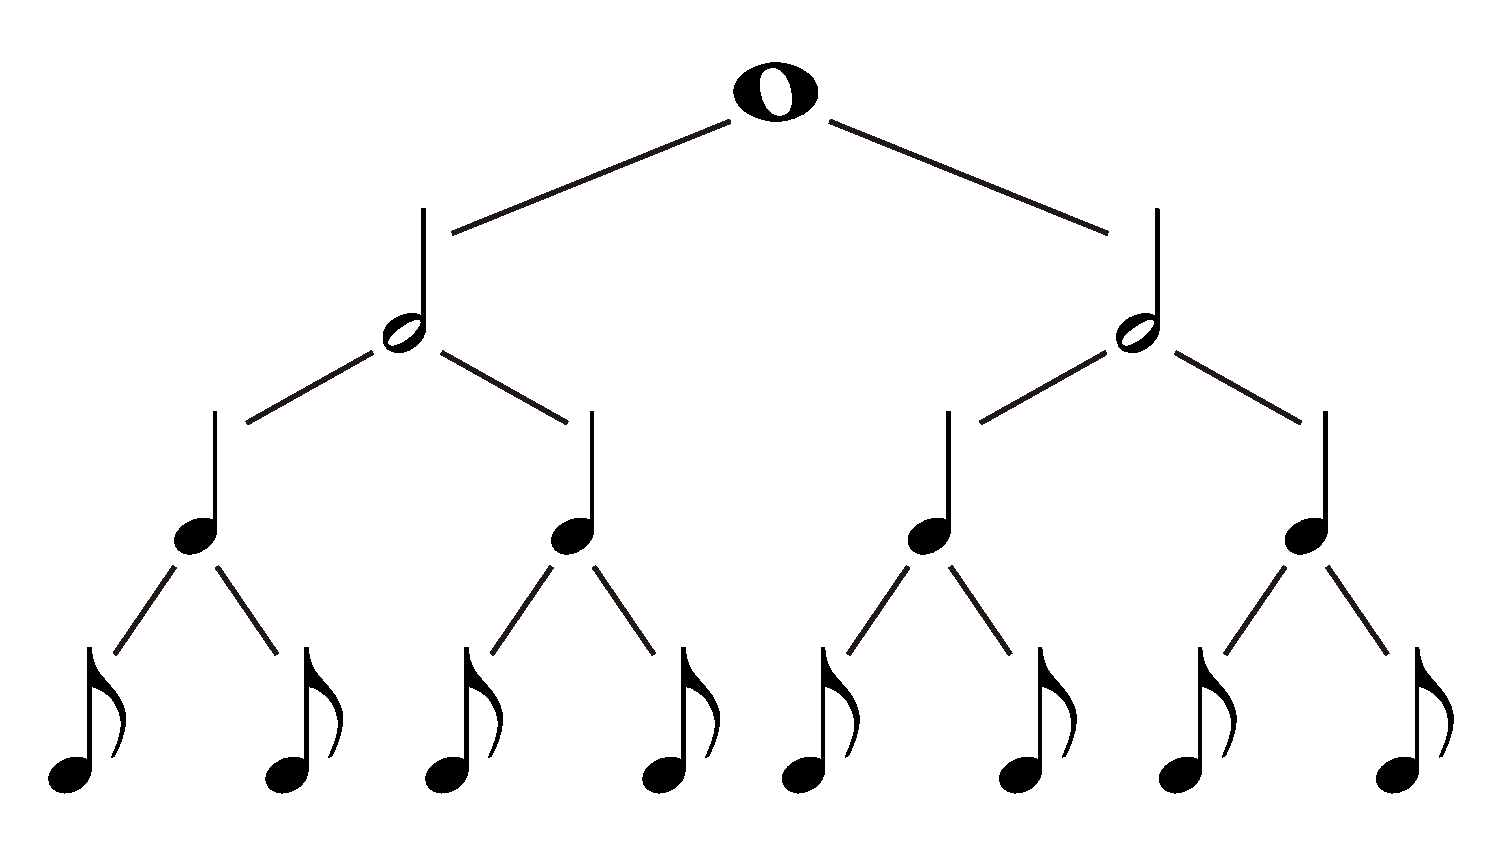
\includegraphics[width=\linewidth]{imagenes/music_tree.pdf}
	\end{frame}
	
	\begin{frame}
		\frametitle{Melody}
		\begin{itemize}
			\item Horizontal dimension of music
			\item Previous notes are previous in time, posterior notes are posterior in time
			\item Pitch is represented by the height at which the note is written, higher position means higher pitch
			\item The pitch of a note matters in relation to the adjacent notes
		\end{itemize}
	\end{frame}
	
	\begin{frame}
		\frametitle{Harmony}
		\begin{itemize}
			\item Vertical dimension of music
			\item Only present in polyphonic pieces or pieces with polyphonic instruments
			\item Two notes of different voices that play at the same time form a chord
			\item The pitch of a note matters in relation to the notes above and below in the other voices
			\item Uses grades of the scale instead of the explicit pitch values of notes to form different chords
		\end{itemize}
	\end{frame}
	
	\begin{frame}
		\frametitle{A little sample}
		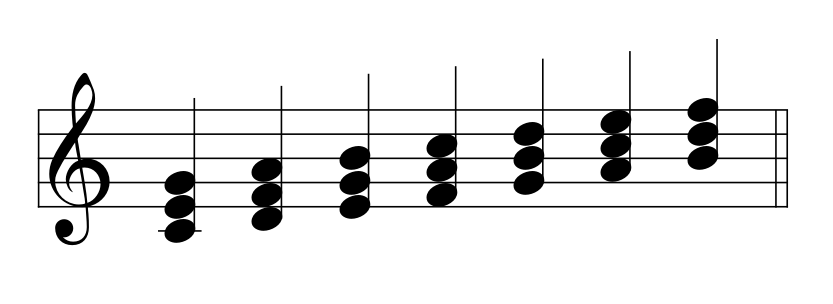
\includegraphics[width=\linewidth]{imagenes/C_chords.png}
	\end{frame}

\section{Demo}
	\begin{frame}
		\frametitle{Demonstration}
		The piece selected for the Demo will be Greensleeves by Henry VII of England. We will see and hear the results of three diffrent processes performed by the tool.
		\begin{itemize}
			\item Harmonization and chord annotation of the score
			\item Given the previous harmonization, the tool will complete a section of the Cello part
			\item Given the previous harmonization, the tool will complete a section of the Violin part
		\end{itemize}
	\end{frame}

\section{The Project}
\subsection{Architecture}
	\begin{frame}
		\frametitle{Initial Architecture}
		\begin{figure}
		\centering
		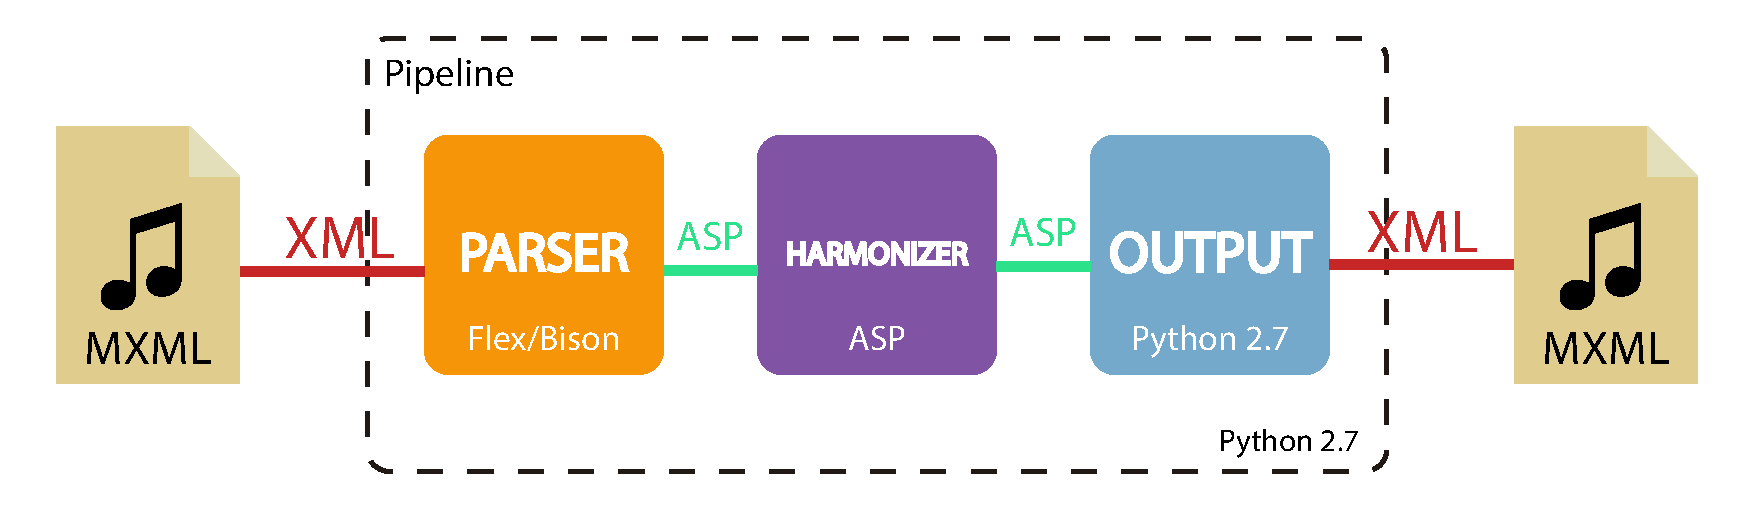
\includegraphics[width=0.8\linewidth]{imagenes/arquitectura_inicial.pdf}
		\end{figure}
	\end{frame}
	\begin{frame}
		\frametitle{Current Architecture}
		\begin{figure}
		\centering
		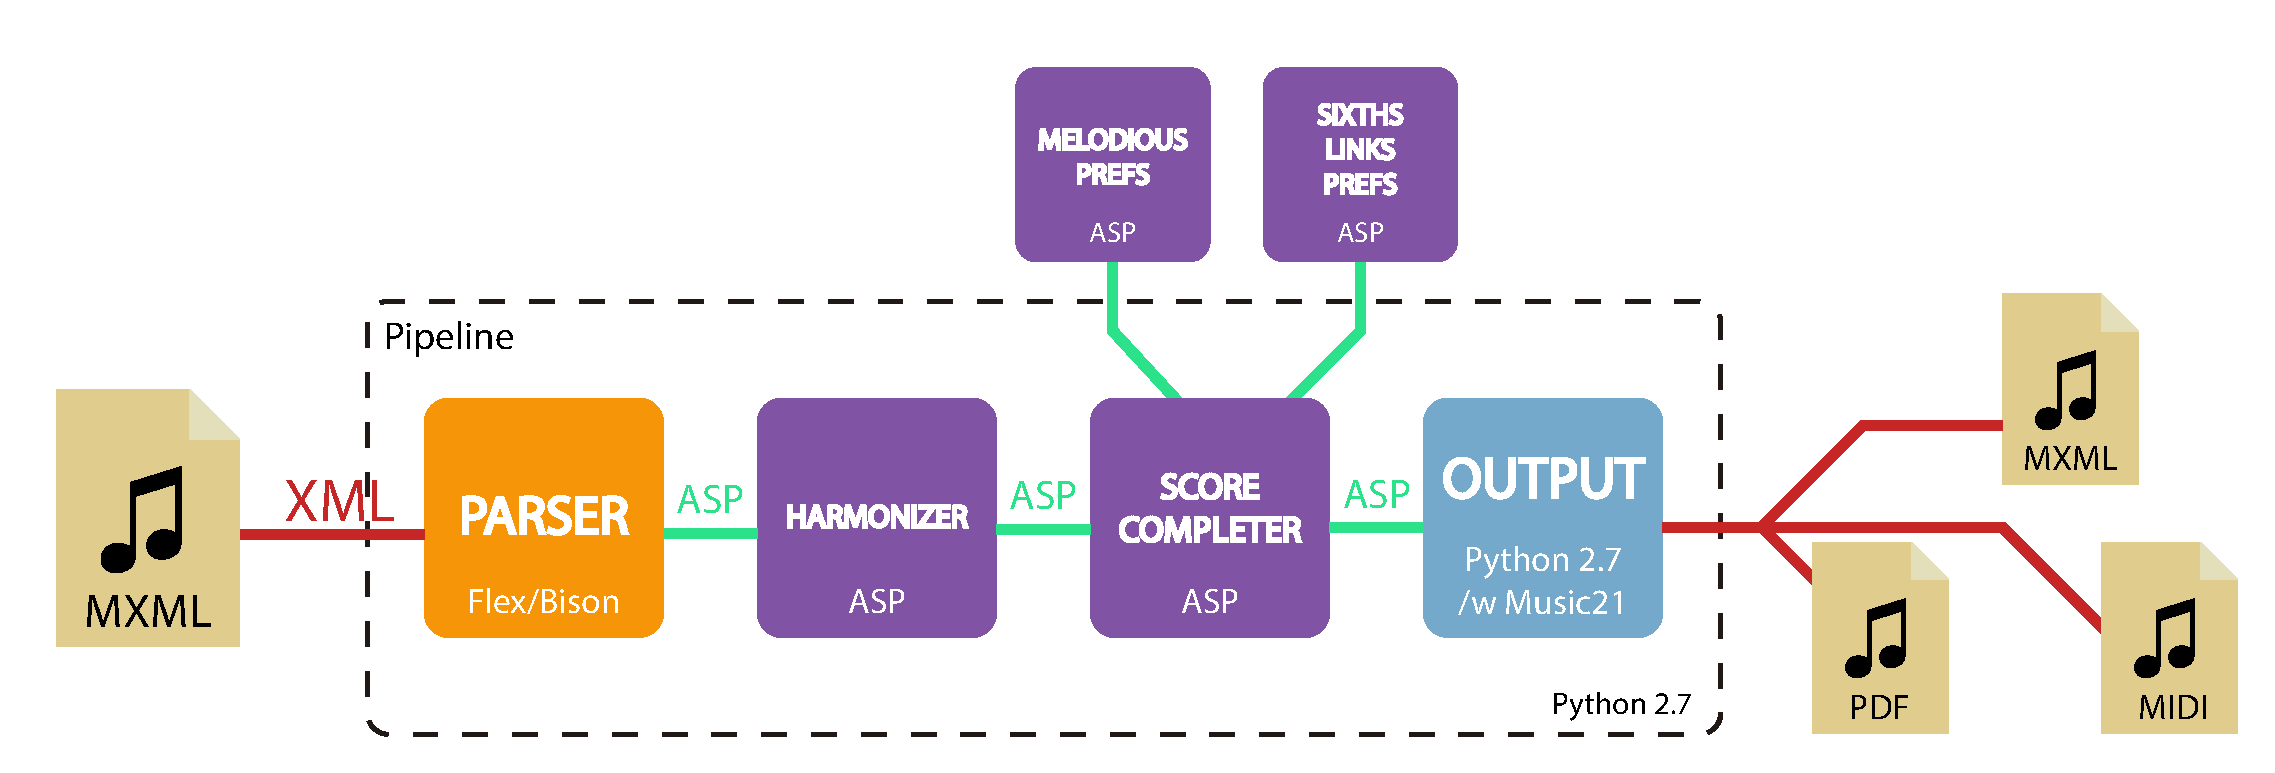
\includegraphics[width=0.8\linewidth]{imagenes/arquitectura_final.pdf}
		\end{figure}
	\end{frame}
\subsection{ASP Core}
	\begin{frame}
		\frametitle{The ASP Core}
		\begin{itemize}
			\item Independent of the solving process and its heuristics
			\item The power of ASP resides in this independence
			\item The problem only needs to be specified by rules and constraints
		\end{itemize}
	\end{frame}
	\begin{frame}[fragile]
		\frametitle{Rules and Constraints}
		\begin{example}[Note Representation]
			\begin{verbatim}
				figure(1,1,22).
				note(1, 72, 22).
			\end{verbatim}
		\end{example}
		\begin{example}[Chord Assignation]
			\begin{verbatim}
				1 { chord(HT,C) : pos_chord(C) } 1 :- htime(HT).
			\end{verbatim}
		\end{example}
		\begin{example}[Score Completion Constraint]
			\begin{verbatim}
				:- freefigure(V,D,FB), ex_grade(V,G1,B1), ex_grade(V,G2,B2),
				   B1 >= FB,B2 >= FB,B1 < FB+D,B2 < FB+D,B1 != B2,G1 != G2.
			\end{verbatim}
		\end{example}
	\end{frame}
	\begin{frame}
	\frametitle{Harmonization}
	\begin{itemize}
		\item Notes are converted to grades of the scale given the key and mode
		\item Chords are assignated to the harmonizable times of the score
		\item Errors are calculated and solver determines the fittest chords for each section.
	\end{itemize}
	\end{frame}
	\begin{frame}
	\frametitle{Score Completion}
	\begin{itemize}
		\item Only used if there are new voices or sections that need to be completed
		\item Given the incomplete or new voices' \textit{tessiturae} notes are assignated to the available positions.
		\item Errors are calculated and solver determines the fittest notes for each time
	\end{itemize}
	\end{frame}
	\begin{frame}
	\frametitle{Melodious Preferences Module}
	\begin{itemize}
		\item Althought not composing melodiously, this module smoothens the output
		\item Checks the tendency of the voices already on the score and makes the new voices imitate them
		\item Smoothens the melodic jumps between notes of a same voice
		\item Reduces the number of consecutive repeated sounds
	\end{itemize}
	\end{frame}
	\begin{frame}
	\frametitle{Sixths Link Preferences Module}
	\begin{itemize}
		\item Progressions of the second inversion of chords are very common in choral music
		\item Creates a per-time harmonization of the score
		\item Finds patterns of second inversion of chords linked in other voices
		\item Tries to continue the progression and creates new progressions of this kind if able
	\end{itemize}
	\end{frame}
	\begin{frame}
	\frametitle{User Configuration}
		The style of the resulting scores produced by the tool is determined by the maximization and minimization of many preferences. These preferences are weighted to be able to specify the significance of each of the measured predicates. Users can define their own preferences by making use of configuration files.
	\end{frame}
\subsection{Input}
	\begin{frame}
	\frametitle{Editors and Formats}
		\begin{itemize}
			\item Scores are edited in an external editor not developed within this project
			\item Musescore 2 was the chosen editor for being free and Open Source
			\item The editor exports the score to a standard music exchange format, MusicXML
			\item MusicXML was chosen among other formats for its parsing simplicity and flexibility
		\end{itemize}
	\end{frame}
	\begin{frame}
	\frametitle{Parser}
		\begin{itemize}
			\item The project also included the development of a little parser
			\item Written in C with the libraries Flex and Bison
			\item Transforms the score in MusicXML to the ASP logic facts that the ASP module uses later
			\item Performs various tasks as:
				\begin{itemize}
					\item Subdivides notes to the length of the smallest figure in the score
					\item Detects most likely key from the score's clef
					\item Reads measure sizes
					\item Transforms chords name above the score to grades
				\end{itemize}
		\end{itemize}
	\end{frame}
\subsection{Pipeline}
	\begin{frame}
	\frametitle{Pipeline}
		\begin{itemize}
			\item Written in Python
			\item Coordinates the different modules secuentially
			\item Gives feedback to the user throught the command line
			\item Allows the user to pick the desired solution for harmonization and score completion
			\item Calls to the internal representation library to store the results of the Harmonization and completion as Python objects.
		\end{itemize}
	\end{frame}
\subsection{Output}
		\begin{frame}
		\frametitle{Output Module}
			\begin{itemize}
				\item Written in Python with the toolkit Music21
				\item Transforms the internal representation of the solution to a Music21 representation
				\item Exports the Music21 representation to the desired format
				\item Some supported formats are Lilypond, PDF, Musescore, MusicXML or MIDI
				\item Allows the result to be saved or directly shown/played
			\end{itemize}
		\end{frame}
\subsection{Results}
	\begin{frame}
	\frametitle{Measured executions results}
	\begin{center}
		\begin{tabular}{ | l | c | c | c | }
			\hline
			Score 			& T. Harmonization 	& T. Measure & T. New Voice \\ \hline \hline
			Greensleeves 	& 1.016s 			& 1.926s	& 4m 49.032s \\ \hline
			Menuet 			& 0.631s 			& 0.726s 	& 3m 50.376s \\ \hline
			Joy to the World& 2.381s 			& 3.813s	& 7m 17.115s \\ \hline
			Twinkle Twinkle & 0.685s 			& 0.716s 	& 2m 31.299s \\ \hline
		\end{tabular}
	\end{center}
	\end{frame}
		\begin{frame}
		\frametitle{Charge Tests}
		\begin{center}
		\begin{center}
				\begin{tabular}{ | l | r | }
					\hline
					Test & Time \\ \hline
					4 measures  & 1.481s \\ \hline
					8 measures 	& 2.394s \\ \hline
					12 measures	& 3.978s \\ \hline
					16 measures & 3.982s \\ \hline
					20 measures & 5.966s \\ \hline
					1 voice & 2m 31.299s \\ \hline
					2 voices & 25m 17.298s  \\ \hline
				\end{tabular}
			\end{center}
		\end{center}
		\end{frame}
\subsection{Future Work}
	\begin{frame}
		\frametitle{Future Work}
		\begin{itemize}
			\item Improve output and correct tiny representation mistakes, althought most of them are expected to be corrected in the 3.0 version of the Music21 toolkit
			\item Implement a plugin interface for MuseScore 2 so the tool can be accessed and manipulated through the editor itself
			\item Improve detection of weak and strong beats of measure
			\item Be able to work with irregular figures such as duplets or triplets
			\item Research about modulation and implement it in the tool
			\item Improve execution times for the inclusion of new voices
			\item Include rhythmic patterning in the new generated voices
			\item Ask for feedback from professional harmony teachers and polish the tool so it can be used in teaching
		\end{itemize}
	\end{frame}
\subsection{Planning and Costs}
	\begin{frame}
		\frametitle{Development Cycle}
		\begin{itemize}
			\item Spiral development with prototypes
			\item SCRUM
		\end{itemize}
	\end{frame}
	\begin{frame}
		\frametitle{Development Costs}
		\begin{table}
		\centering
			\begin{tabular}{ | l | c | c | c |}
				\hline
				\textbf{Profile} & \textbf{Cost/Hour} & \textbf{Hours} & \textbf{Total} \\ \hline
				Student & 5.5\euro{} & 362 & 1991\euro{} \\ \hline
				Director  & 9\euro{} & 12 & 108\euro{} \\ \hline
				\textbf{Total} & & & 2099\euro{} \\ \hline
			\end{tabular}
		\end{table}
	\end{frame}
	\begin{frame}
		\frametitle{Iteration Breakdown}
		\begin{figure}
		\centering
		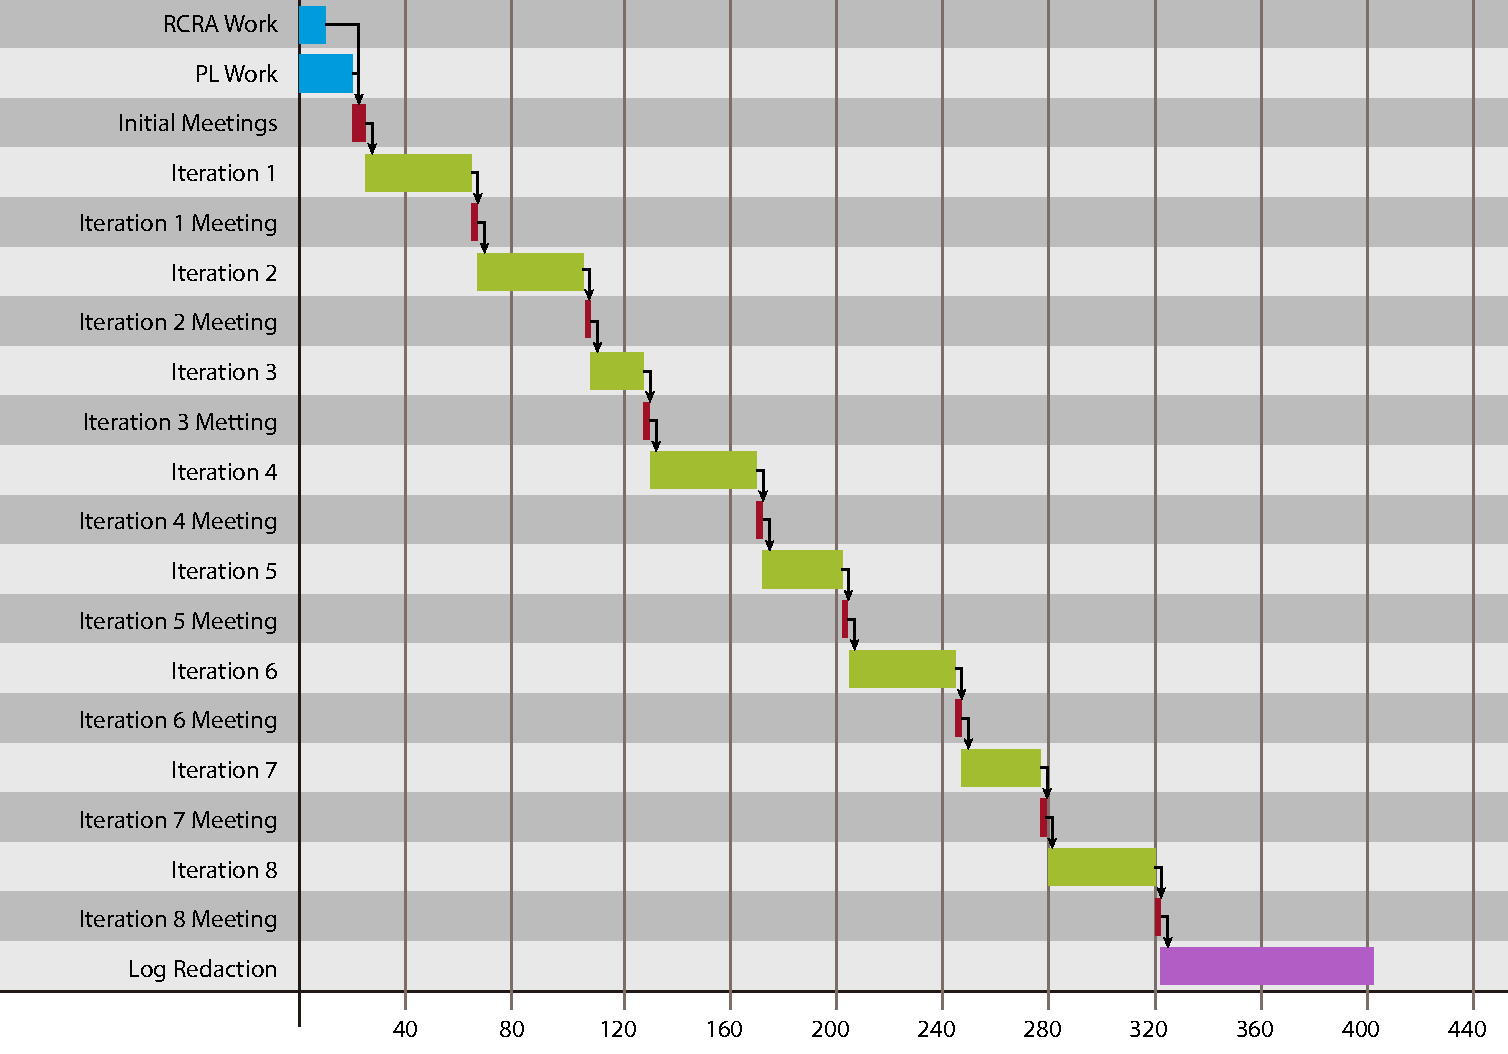
\includegraphics[width=0.8\linewidth]{imagenes/diagrama_tareas.pdf}
		\end{figure}
	\end{frame}
\subsection{Conclusions}
		\begin{frame}
			\frametitle{Conclusions}
			\begin{itemize}
			      \item<pro@1-> Achieved the main goals of the project and extended some of the functionality
			      \item<pro@1-> The tool produces correct scores in good times
			      \item<con@1-> The interface is pretty poor
			      \item<con@1-> User still needs informatic knowledge to use it
			    \end{itemize}
			 The project as it is now needs more work to achieve full usability and be able to reach the target it's intended to. Despite this, the project works really great and demonstrates once again the validity of ASP to many aspects of life, such as music.
		\end{frame}
\begin{frame}
\titlepage % Print the title page as the first slide
\end{frame}


\end{document} 